The first round of testing was to ensure that the odometry was working properly; the first data set is the location dereived solely from odometry data.

\begin{figure}
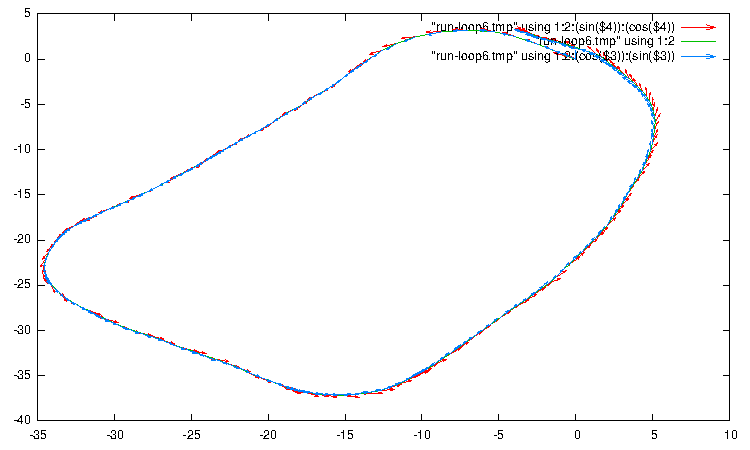
\includegraphics{run-loop6}
\caption{Odometry from a loop}
\end{figure}

For the second round of testing, I wrote a program to give the robot four points in a square, so that it would drive in a roughly square-shaped loop and return to its starting point. The data shows the robot's position estimate, including uncertainty, and the path plotted by raw odometry data.

\begin{figure}
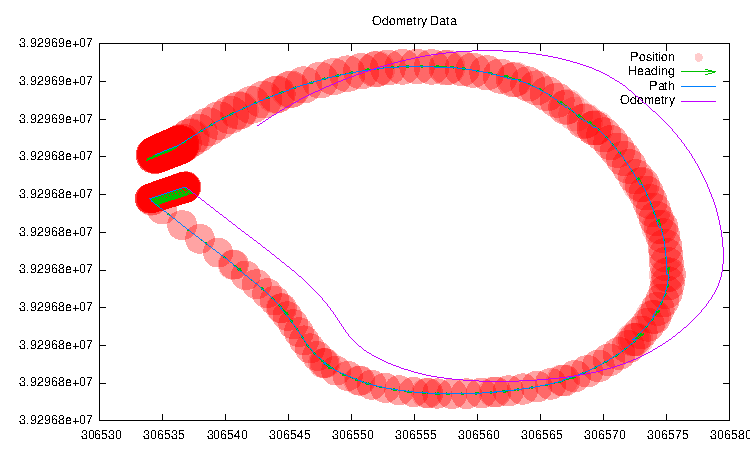
\includegraphics{run-2011-05-30-3}
\caption{Odometry and position output from square test}
\end{figure}


\begin{tabular}{ | p{0.4\textwidth} | p{0.4\textwidth} | }
        \hline
        \textbf{Test Description} & \textbf{Results} \\
           \hline
           \textbf{Odometry loop closure:} manually drive a small loop, about 20-30 meters in circumference, and return to the robot's starting position & Odometry reports final position within 0.5 meters of start position. \\
              \hline
\textbf{Square test:} autonomously drive to the four points of a square and return to the starting position. The square is 3 meters to a side. & Final position off by 1-2 meters. \\
       \hline
\textbf{Dexter Lawn loop:} Given the coordinates of the corners of dexter lawn, drive around the lawn and return to the starting position. & Successfully completed a lap without running into any obstacles. Final position off by 4-5 meters \\
       \hline
\end{tabular}
